\chapter[Referencial Teórico]{Referencial Teórico}

\section{Teorias de Aprendizagem}

Para qualquer profissional na área de ensino e aprendizagem, é necessário o estudo das teorias de aprendizagem, no caso específico deste trabalho, foi utilizada a teoria Cognitivista, que serviu como suporte teórico para a modelagem das redes de vídeos interativos utilizadas no sistema.

Segundo \cite{moreira1999}, as teorias de aprendizagem são tentativas de interpretar sistematicamente, organizar e prever os conhecimentos relativos à aprendizagem. Hill (2002) representa as teorias como o ponto de vista sobre a abordagem de assuntos relativos ao aprendizado e a especificação de quais são as variáveis independentes, dependentes e intervenientes que possuem relevância acadêmica.

As teorias behavioristas, ou comportamentalistas, são aquelas ligadas fundamentalmente aos comportamentos observáveis e mensuráveis do indivíduo, tendo como ideia inicial e fundamental o uso de estímulos e respostas.

Concebido por John B. Watson, o behaviorismo rejeita a hipótese de que existe algo além do mundo físico. Se opondo à psicologia da época que estudava os sentimentos e pensamentos das pessoas, o behaviorismo estava centrado no que as pessoas faziam e que era observável \cite{moreira1999}.

Segundo o behaviorismo radical, ou Skinneriano, o estímulo é o evento que afeta os sentidos do aprendiz, o reforço é o evento que aumenta a probabilidade de ocorrência de um evento que o precedeu, e as contingências do reforço são um arranjo de uma situação que favoreça a ocorrência de uma resposta que leve ao reforço. O comportamento respondente é aquele que é eliciado involuntariamente (p.ex. contração da pupila sob incidência de luz). O comportamento operante é aquele em que o aprendiz opera sobre o meio conscientemente, agrupando a maior parte dos comportamentos humanos. Semelhantemente, são definidos os condicionamentos como operantes ou respondentes, já que para todo comportamento existe um condicionamento \cite{fragelli2010, silva2005}. 

Em termos de aplicações educacionais, Skinner acreditava que o papel do professor está muito mais ligado às contingências de reforço do que ao par estímulo-resposta. Em outras palavras, o professor deve atuar no planejamento de um contexto que aumente a probabilidade do comportamento desejável acontecer. Vários fenômenos estudados por Skinner podem ser aplicados ao processo educacional, como o a modelagem e o esmaecimento.

A modelagem, ou método das aproximações sucessivas, consiste no reforço de várias respostas intermediárias que servem como uma ponte para um comportamento desejado. No esmaecimento, são utilizados diferentes estímulos em conjunto com o que se deseja alcançar, tais estímulos são esmaecidos até que se mantenha apenas o desejável.

Apesar de trazer pontos relevantes para aplicação no ensino e aprendizagem, a posição radical e inflexível de Skinner em relação ao behaviorismo e suas convicções levaram-no a ignorar completamente a psicologia cognitiva, o que culminou no declínio do behaviorismo radical \cite{fragelli2010, silva2005, moreira1999}.

Por volta de 1975 as pesquisas sobre a psicologia cognitiva começaram a superar as pesquisas behavioristas em número de publicações. Em parte, essa ascensão se deve ao fato de que o behaviorismo não explicava a complexidade do comportamento humano, se restringindo a usar estímulos, reforços e respostas \cite{robins1999}.

A cognição, ou atividade mental, representa a aquisição, o armazenamento, a transformação e aplicação do conhecimento. A abordagem cognitiva é uma orientação teórica que enfatiza o conhecimento que as pessoas possuem e seus processos mentais \cite{matlin2004}.

A teoria cognitiva de \cite{ausubel2000} está centrada no conceito de aprendizagem significativa, para a qual o cerne da aprendizagem está no que o aprendiz já conhece, sendo que, para o aprendizado e retenção de algo novo em sua estrutura cognitiva, é necessário que existam conceitos prévios que atuem como âncoras para esse novo conceito formado.

O conceito subsunçor, ou simplesmente subsunçor, é este conceito âncora já existente na estrutura cognitiva do indivíduo, com o qual um novo conceito aprendido interage. Além disso, quando um novo conceito é ancorado ao subsunçor, ele se torna mais desenvolvido e inclusivo, mas se a aprendizagem não ocorre com frequência em conjunto com um subsunçor, ele se torna limitado e menos desenvolvido.

Com isso, se a aprendizagem significativa necessita da existência de conceitos subsunçores, é necessário então que em um momento inicial, ocorra uma aprendizagem mecânica, que independe de conceitos prévios. Nesse sentido, principalmente na educação infantil, a aprendizagem mecânica é o ponto inicial para a aprendizagem significativa, com o desenvolvimento da estrutura cognitiva, os conceitos vão se tornando mais elaborados e abrangentes, permitindo maior ocorrência da aprendizagem significativa \cite{ausubel2000}.

Segundo Ausubel, é mais fácil para um indivíduo aprender significativamente termos mais amplos e inclusivos para depois captar conceitos mais específicos como uma diferenciação do todo, do que aprender as partes para se chegar ao todo. Assim, Ausubel apresenta teorias como a diferenciação progressiva, que deve ser um princípio programático do material de ensino, e a reconciliação integrativa para explorar as similaridades e diferenças entre as ideias para se propor uma nova instrução \cite{ausubel2000, fragelli2010}. 

Já os organizadores prévios são estruturas facilitadoras do processo de aprendizagem significativa, sendo geralmente materiais introdutórios que possuem alto nível de abstração, generalidade e inclusividade, e servem como uma ponte cognitiva entre o que o indivíduo conhece e o que se pretende aprender, promovendo uma disposição do sujeito a aprender significativamente o conteúdo \cite{ausubel2000, tavares2010}.

Nesse sentido, os organizadores prévios são particularmente especiais para a confecção de materiais digitais e interativos de aprendizagem, e têm tido sucesso em projetos nacionais e internacionais \cite{tavares2010, novak2006}. Neste trabalho, os vídeos Interativos servem como mecanismo para utilização dessa teoria, no sentido de permitirem a construção gradual do conteúdo a ser aprendido.


\section{Princípios do Aprendizado Multimídia}

\cite{mayer2001} define os princípios do aprendizado de multimídia tendo como base a teoria da codificação dual. \cite{paivio1986} distingue o aprendizado por imagens e animações do aprendizado pela escuta, e afirma que o canal que processa imagens é diferente do canal que processa o som e ambos têm capacidades limitadas \cite{tavares2010}.

Além disso, Mayer afirma que para que ocorra aprendizagem significativa, ambos os canais requerem um processamento cognitivo, no qual imagens e palavras são processadas, organizadas e conectadas segundo uma ordem lógica para a formação de um conceito, como ilustrado na figura \ref{fig:aprendizado} \cite{mayer2001, moreno2000}. Nesse sentido, alguns princípios para a construção de materiais multimídia estabelecidos pela literatura foram levados em consideração para a modelagem abordada neste trabalho, sendo eles: segmentação, pré-texto, modalidade e diferenças individuais \cite{clark2011, mayer2001, moreno2000}, explicados a seguir.

\begin{figure}[h!]
	\centering
  	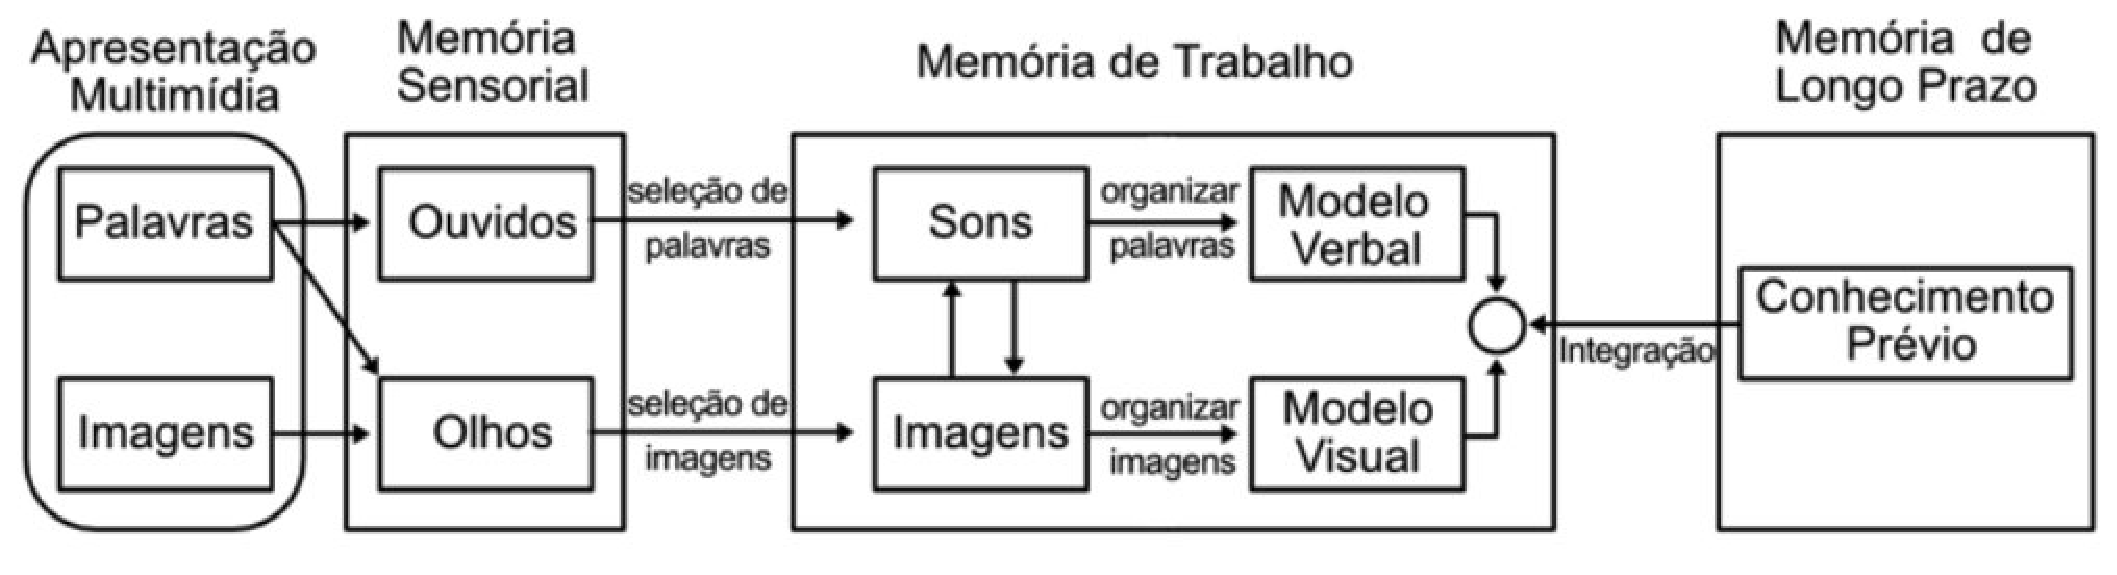
\includegraphics[width=.9\linewidth]{figuras/aprendizado.eps}
  	\caption{Teoria cognitiva para a aprendizagem multimídia}
  	\small{Fonte: \cite{moreno2000}}
  	\label{fig:aprendizado}
\end{figure}

O princípio da segmentação diz que o estudante aprende melhor quando um conteúdo é apresentado em vários vídeos, ou segmentos de um mesmo vídeo, do que quando é utilizado um único vídeo contínuo ininterrupto. A justificativa é que, para o aluno, o processamento cognitivo muitas vezes não acompanha o fluxo de informações contínuo para que ocorra aprendizagem significativa, o que diminui a capacidade do aprendiz de armazenar a informação passada \cite{mayer2001, moreno2000}.

O princípio do pré-texto diz que um estudante aprende melhor se conhecer os conceitos e tópicos que serão estudados no curso antes da apresentação do conteúdo \cite{clark2011}. Esse princípio valoriza a utilização de tabelas ou mapas conceituais para que o estudante possa organizar os conceitos antes da definição dos mesmos, estando diretamente relacionado a teoria da apresentação "Todo-Parte" que afirma que um estudante aprende melhor quando conhece o todo antes das partes \cite{mayer2014, mayer2001}, esta última tem como base a teoria cognitiva das diferenciações sucessivas \cite{ausubel2000}.

O princípio da modalidade afirma que o aprendizado é mais efetivo quando se utiliza animação e narração se comparado com o uso de animação e texto escrito. Dessa forma, devem ser valorizados discursos com representação visual e o não uso de textos explicativos simultaneamente \cite{mayer2014}.

O princípio das diferenças individuais afirma que a modelagem do material multimídia afeta muito mais estudantes de níveis inferiores do que estudantes mais avançados. Esse princípio diz então que a modelagem deve ser mais direcionada para estudantes de menor nível \cite{mayer2014} ou então, pode-se utilizar uma adaptação do conteúdo para adequar o material aos diferentes níveis de estudantes \cite{fragelli2010, brusilovsky1996, brusilovsky1994}, como abordado neste trabalho.

\section{Sistemas de Hipermídias Adaptativas}



\section{Quantização de Redes por Nodos}


